\tikzset{highlight/.style={orange!75!white,line width=6pt,line cap=round}}
%\tikzset{highlight2/.style={tngreen!80,line width=11pt,line cap=round}}
\tikzset{highlight2/.style={tngreen!70!yellow!60,line width=11pt,line cap=round}}
\tikzset{psline/.style={decorate,decoration={amplitude=0.3mm,segment length=2mm,post length=1.5mm,pre length=1.5mm,coil,aspect=0}}}
\tikzset{plainlin/.style={line width=1pt}}
\def\shortendistance{5pt}
\tikzset{plainlin shorten/.style={line width=1pt,shorten >=\shortendistance,shorten <=\shortendistance}}

\tikzset{lin shorten/.style={shorten >=\shortendistance,shorten <=\shortendistance,line width=1pt,decoration={markings, mark=at position 0.5*\pgfdecoratedpathlength+1.8pt with {\arrow{angle 90}}}, postaction={decorate}}}
% Name of file with picture %%%%%%%%%%%%%%%%%%%%%%%%%%%%%%%%%%%%%%%%%%%


\usetikzlibrary{calc,decorations.markings,decorations.pathmorphing,arrows,external,decorations.pathreplacing,arrows.meta,calc,decorations.markings,decorations.pathmorphing,shapes}

\newcommand{\vertexat}[1]{\fill [very thick,draw=white,fill=black] #1 circle (3pt);}


\definecolor{tnred}{RGB}{     255, 63,   63}
%\definecolor{tnorange}{RGB}{  255, 204,   6}
% #ecb939	()
\definecolor{tnorange}{RGB}{  220, 140,   6}
\definecolor{tnblue}{RGB}{     10, 154, 215}
\definecolor{tngreen}{RGB}{   114, 165,  10}
\definecolor{tnmagenta}{RGB}{ 215,  10, 154}
\definecolor{tnbg}{RGB}{252,252,252}
\definecolor{tnfg}{RGB}{5,8,12}

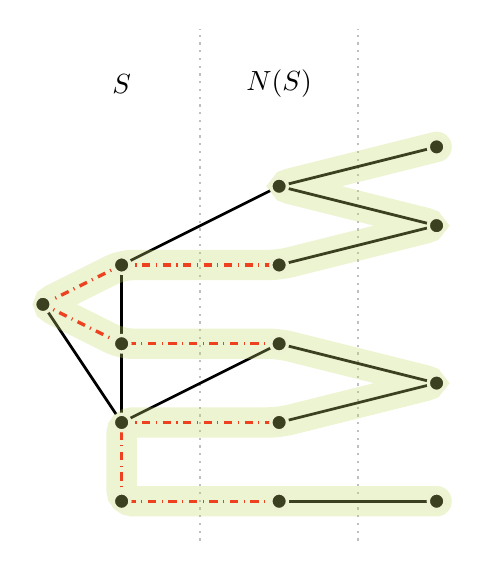
\begin{tikzpicture}

    \node at (1,4.3) {$S$};
    \node at (3,4.3) {$N(S)$};

    \draw [dotted,thick,gray!50] (2,-1.5) -- (2,5);
    \draw [dotted,thick,gray!50] (4,-1.5) -- (4,5);

\def\midx{3}
    \coordinate (a) at ($(5,-1)$);
    \coordinate (b) at ($(\midx,-1)$);
    \coordinate (c) at ($(1, -1)$);
    \coordinate (d) at ($(1, 0)$);
    \coordinate (e) at ($(\midx, 0)$);
    \coordinate (f) at ($(5, .5)$);
    \coordinate (g) at ($(\midx, 1)$);
    \coordinate (h) at ($(1, 1)$);
    \coordinate (i) at ($(0,1.5)$);
    \coordinate (j) at ($(1,2)$);
    \coordinate (k) at ($(\midx,2)$);
    \coordinate (l) at ($(5,2.5)$);
    \coordinate (m) at ($(\midx,3)$);
    \coordinate (n) at ($(5,3.5)$);

    \draw [plainlin] (a) -- (b);
    \draw [dashdotted, very thick,red] (b) -- (c);
    \draw [dashdotted, very thick,red] (c) -- (d);
    \draw [dashdotted, very thick,red] (d) -- (e);
    \draw [plainlin]%,gray!40,line width=1.5pt]
    (d) -- (h);
    \draw [plainlin]%,gray!40,line width=1.5pt]
    (d) -- (i);
    \draw [plainlin]%,gray!40,line width=1.5pt]
    (d) -- (g);
    \draw [plainlin] (e) -- (f);
    \draw [plainlin] (f) -- (g);
    \draw [dashdotted, very thick,red] (g) -- (h);
    \draw [dashdotted, very thick,red] (h) -- (i);
    \draw [plainlin]%,gray!40,line width=1.5pt]
    (h) -- (j);
    \draw [dashdotted, very thick,red] (i) -- (j);
    \draw [dashdotted, very thick,red] (j) -- (k);
    \draw [plainlin]%,gray!40,line width=1.5pt]
    (j) -- (m);
    \draw [plainlin] (k) -- (l);
    \draw [plainlin] (l) -- (m);
    \draw [plainlin] (m) -- (n);

    \foreach \nn in {a,b,c,d,e,f,g,h,i,j,k,l,m,n} {
      \vertexat{(\nn)}
    }

    \draw [highlight2,rounded corners,line cap=round,opacity=0.3] (a) to (b) to (c) to (d) to (e) to (f) to(g) to (h) to (i) to (j) to (k) to (l) to (m) to (n);;

\end{tikzpicture}
